\documentclass[conference]{IEEEtran}
\usepackage{amsmath,amssymb,amsfonts}
\usepackage{url}
\usepackage{subfigure}
\usepackage{booktabs,threeparttable,multirow}
\usepackage{siunitx}
\usepackage{pgfplots}
\usepackage{graphicx}
\graphicspath{ {images/} }

% new math operators
\DeclareMathOperator{\abs}{abs}

% todo command
\usepackage{marginnote}
\newcounter{todocnt}
\newcommand{\Sim}{\textsc{Simon}} 
\setcounter{todocnt}{0}
\newcommand{\todo}[1]{\stepcounter{todocnt}{\tt {[#1]}} \marginpar{{$\blacksquare$ \thetodocnt}}}  
\newcommand{\specialcell}[2][c]{%
  \begin{tabular}[#1]{@{}c@{}}#2\end{tabular}}

\hyphenation{op-tical net-works semi-con-duc-tor}
\IEEEoverridecommandlockouts

\author{Dolan Murvihill \and Nathan Wells}

\usepackage{siunitx}

\newcommand{\latin}[1]{
    \textit{#1}
}
\newcommand{\name}[1]{
    \textit{#1}
}
\uchyph=0 % prevent capitalized words like names from being hyphenated



\begin{document}

\title{Countermeasures against co-location attempts in the cloud}


\author{\IEEEauthorblockN{Dolan Murvihill, Nathan Wells
}
\IEEEauthorblockA{Worcester Polytechnic Institute, 
Worcester, MA 01609, USA\\
Email: \texttt{\{dm, nhwells\}@wpi.edu}
}}
\maketitle
\nocite{*}

\begin{abstract}
Recent research has demonstrated that cloud services such as Amazon AWS do not provide perfect isolation~--- that there
  are side channels between virtual machines that reside on the same host.
In particular, it is possible, under some circumstances, to use cache timing information to perform a full AES key
  recovery against a VM sharing the same cache.

Other work has shown that cloud services such as Amazon AWS provision virtual machines using straightforward, often
  predictable algorithms, and others have demonstrated that it is possible to achieve the required co-location to
  perform a co-location attack.
We would like to discern whether Amazon AWS has implemented any countermeasures against co-location attacks since the
  first successful cloud co-location six years ago.
We repeated one aspect of a previous successful attack, and found that, surprisingly, the same attack vector continues
  to be plausible.
\end{abstract}

\section{Motivation}

\begin{itemize}
  \item Amazon's EC2 service is very popular and used for by variety of customers, some of which have sensitive data.
  \item This makes VMs on EC2 a worthwhile target.
  \item Ristenpart et al. have demonstrated that it is possible to create a VM co-resident with a target instance and
    that existing side-channel attacks can be employed against co-resident instances on the cloud.
  \item We expect that Amazon has since adjusted their VM location algorithms to make the Ristenpart attack more
    difficult. We would like to assess the current viability of the Ristenpart attack on today's AWS.
\end{itemize}

\section{Background}\label{sec:background}
The idea of performing cryptanalytic attacks against co-located virtual machines was discussed by Ristenpart, Shacham,
  and Savage in 2009 \cite{ristenpart2009cloud}.
They measure co-location success rates in Amazon Web Services (AWS), and suggest some potential attacks against
  co-located VMs.
Zhang \cite{zhang2014cross} et al. presented a cross-VM attack using Ristenpart's attack which was able to recover an El Gamal key across
Xen VMs.
Irazoqui, Inci, Eisenbarth, and Sunar \cite{irazoqui2014wait} then presented a practical, fast, and realistic full key
  recovery against AES across virtual machines, based on Bernstein's \cite{bernstein2005cache} attack.

Research into co-location attacks and cross-VM attacks continues to be an active research area.

\section{Work Description}
We reproduced two parts of the Ristenpart attack: first, a ``network cartography'' project that tried to find
  correlations between AWS instance creation parameters and IP address; and second, a ``covert channel'' approach to
  verifying co-location.
Our goal is to determine whether one of our instances shares a virtual machine with an arbitrary AWS instance.

\subsection{Network Cartography}
In this section, we create a “map” of instance placements by recording the private IP address of the instances after placing them.
Our hope is this will give insight into how target instances are placed.
This will help in the attempt to establish co-residence with these target instances.

From published information about EC2, we know that each availability zone has its own dedicated hardware. 
Using this and the cartography information in Ristenpart, we hypothesize that each zone will have its own 
range of internal IP addresses. 
We also hypothesize that instances of the same type would fall in the same internal IP address ranges. 
If these hypotheses are correct, an attacker could achieve co-location much more easily by finding the internal 
IP address of the target and launching instances with similar parameters. 
Amazon’s DNS service can be used to obtain this address from the public IP address of the target.

We test our theory by launching a number of instances with different types in each availability zone. 
We then attempt to create a set of rules that describe the likely availability zone and instance type of a given 
private IP address.  
With the data collected, we create a “map” of IP addresses and instance parameters that can be used to determine 
a target’s parameters.

All instances were launched in US West 2 zones a, b, and c. The t2.micro, small, and medium instance types 
were used. 
Of the 1011 instances launched, all fell into the same /16 prefix (172.31.0.0). 
Instances were launched 
in groups of 3 or 5 of each type. 
We observed that instances of the same type launched sequentially had consecutive IP addresses, which is called 
sequential placement locality. 

While it was fairly likely that instances launched in the same zone would be placed together based on previous 
work and knowledge of the inner workings of EC2, we were surprised to see that different instances types were launched 
very close to each other (within the same /24 prefix). 
Of the 48 /24 prefixes observed across the three availability zones, the vast majority contained more than one 
instance type. 
Additionally, a small number of m3.medium, large, and xlarge instances were launched which all fell into the same 
/20 prefix as other instances in that zone.

The following plots show the results of the data collected. 
IP addresses are represented by their integer representation minus 2887712768, which represents the first address 
(172.31.0.0). 
Zone 2c occupied the 172.31.0.0/20 prefix, Zone 2a occupied 172.31.16.0/20, and Zone 2b occupied 172.31.32.0/20. 
In (this figure), the zones are numbered one to three, with a being one.
%\begin{figure}[h]
%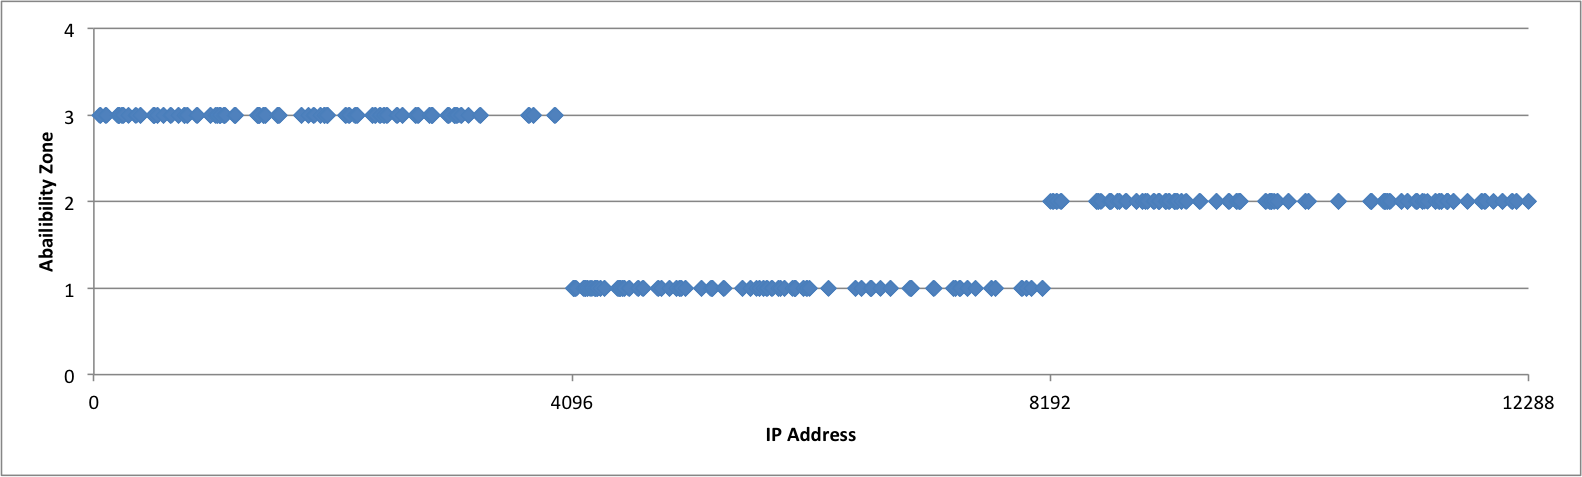
\includegraphics[scale=.5]{zoneIP}
%\caption{Plot of private IP address vs availability zone}
%\end{figure}
In (these figures), the distribution of instance types in each zone is showed. The instances are numbered from 
one to three, for t2.micro, t2.small, and t2.medium instances respectively.
%\begin{figure}[h]
%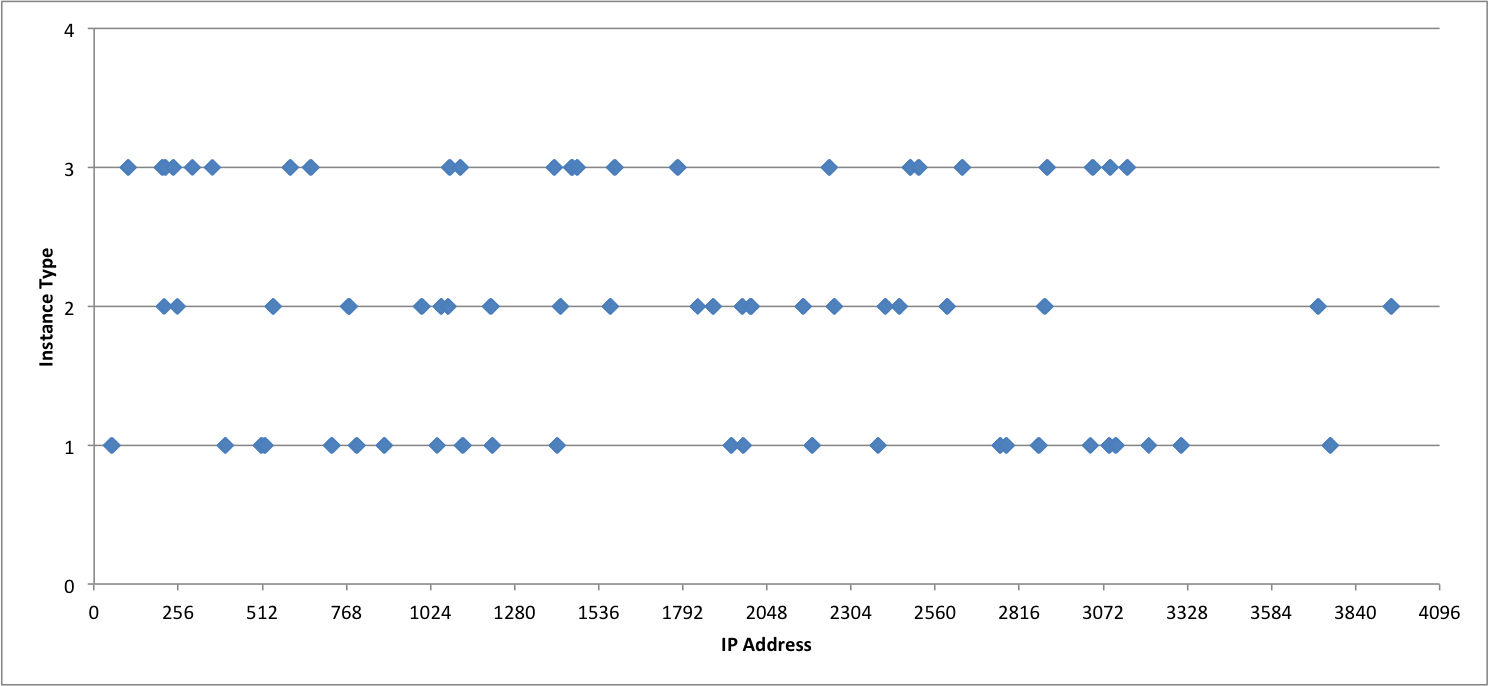
\includegraphics[scale=.5]{2cTypeIP}
%\caption{Plot of private IP address vs instance type in Zone 2c}
%\end{figure}
%\begin{figure}[h]
%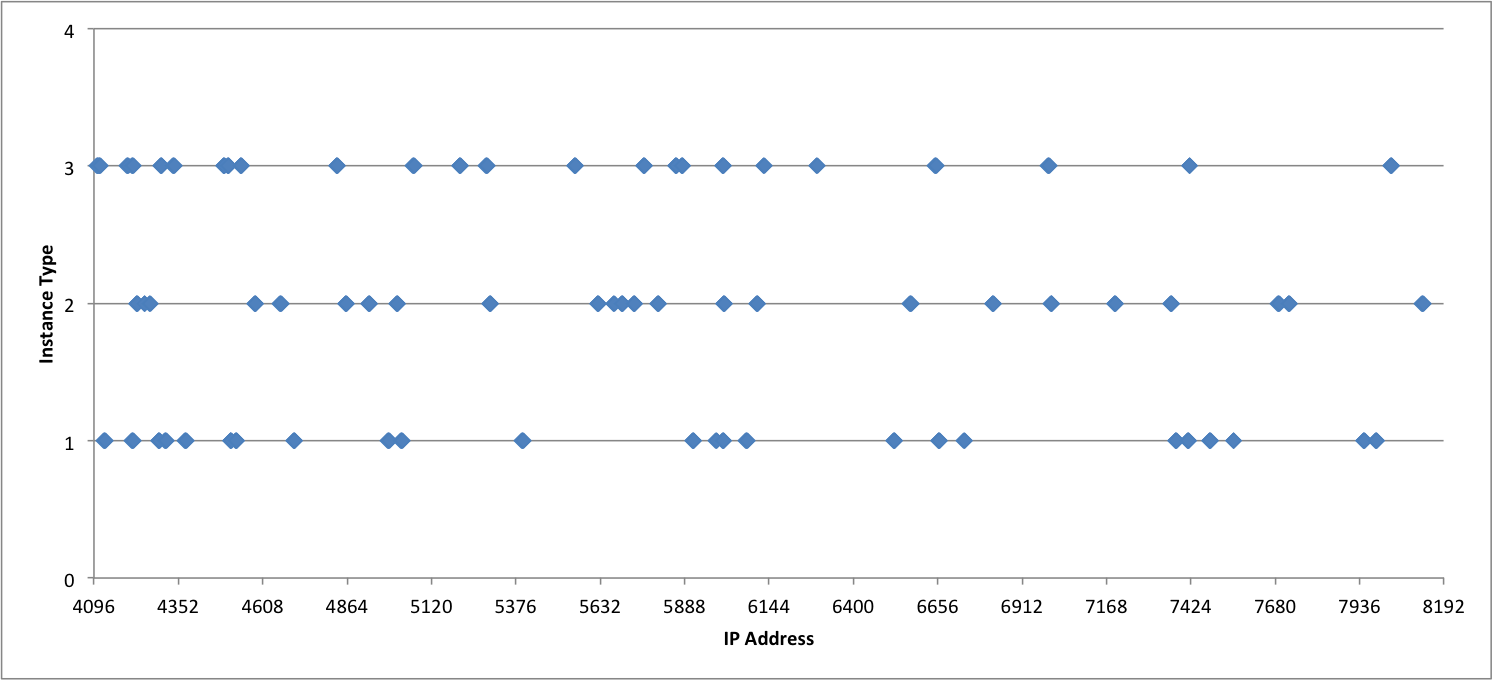
\includegraphics[scale=.5]{2aTypeIP}
%\caption{Plot of private IP address vs instance type in Zone 2a}
%\end{figure}
%\begin{figure}[h]
%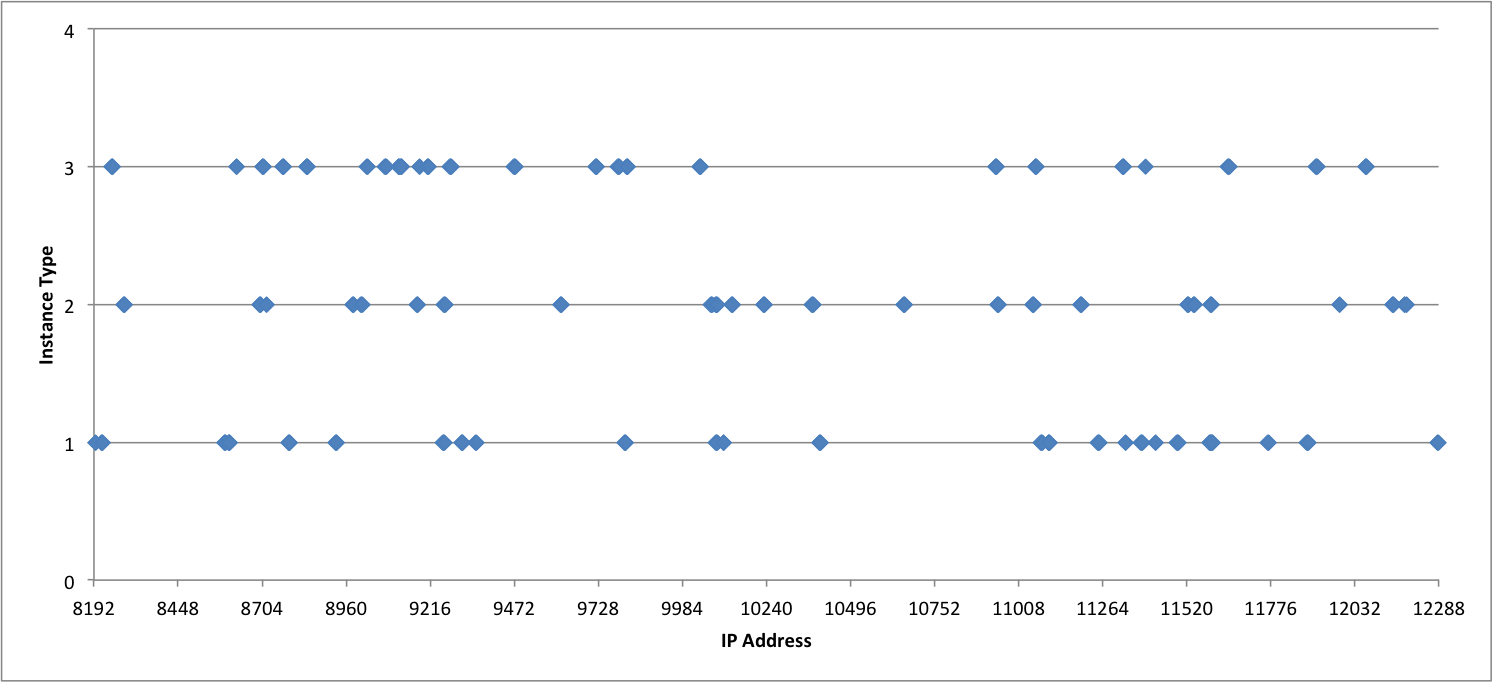
\includegraphics[scale=.5]{2bTypeIP}
%\caption{Plot of private IP address vs instance type in Zone 2b}
%\end{figure}
Our goal is to be able to discern co-location with an arbitrary instance, but we can begin by attempting to discern
  co-location with another instance under our control.
Ristenpart et al. evaluated co-location by attempting to transmit data across a covert channel between two virtual
  machines --- in their case, by causing seeks and measuring seek times. Our approach is essentially the same.
A ``sender'' process continually reads values from random locations on the disk to send a one, and does nothing to
  send a zero.
A ``receiver'' process is constantly reading values, and measuring the seek times.
If the processes shared a hard drive (and thus, a host), the receiver process would be expected to observe consistently
  higher seek times while the sender is transmitting ones than while the sender is transmitting zeroes.
Thus, successfully transmitting a message across this secret channel would imply that the virtual machines are
  co-located.

\subsubsection{Verification on Local Machine}
Some calibration measurements were taken to make sure that the covert channel approach would work.
The ``seeker'', a short C program, was adapted from a 2007 Linux Insight article \cite{seeker07} to provide the seek
  capability and measurement.
The seeker read random locations from the disk as frequently as possible for thirty seconds, then reported the mean
  time required for each reading.
The seeker was run one hundred times on a personal computer belonging to one of the authors, and the mean seek time
  from each sample was recorded.

A similar test was performed on the same personal computer that ran two seekers at once.
One hundred samples were taken from one seeker (the ``receiver'').
The other seeker's samples were discarded.

\subsubsection{Calibration on AWS}
Once we were satisfied that the seeker was performing as expected, we used it to calibrate the covert channel on a
  t2.micro AWS instance.
The one-seeker test and two-seeker test were each run one hundred times, and their sampling distributions were
  used to set the mean seek time ranges that corresponded to zero and one.

\section{Results}
\subsection{Covert Channel}
The tests we ran on our personal computer, described in Section~{mth:localcc} provided information that gave us high
  confidence in the validity of the results we measured on AWS.

Even if the probability distribution of the hard drive seek time was not Gaussian, such a large number of samples were
  taken that the sampling distribution of means can be treated as Gaussian, according to the Central Limit Theorem.

The distributions are very narrow and widely separated, giving us high confidence in the accuracy of our message
  transmission.
The sampling distribution of mean seek time in the single-seeker test (transmitting zeroes) was centered on
  \SI{13.36}{ms}, with a standard deviation of \SI{0.36}{ms}.
For the double-seeker test (transmitting ones), the center was \SI{24.08}{ms} with a standard deviation of
  \SI{1.42}{ms}.
Based on these calibration figures, we could read a mean seek time between \SI{11.56}{ms} and \SI{15.16}{ms}
  as a zero, and a mean seek time between \SI{16.98}{ms} and \SI{31.18}{ms} as a one, and accomplish an error rate of
  \SI{3e-7} errors per bit transmitted.

Our first calibration test on AWS produced an unexpected result; the first \num{53} samples of the one-seeker test gave
  a mean seek time between \SI{0.29}{ms} and \SI{0.31}{ms}, while the last \num{46} were all over \SI{36}{ms}.
Sample \num{54} gave a mean of \SI{0.81}{ms}, indicating that toward the end of that sample, some condition changed
  that affected the seek time of the VM.
The two-seeker test, which ran after the one-seeker test, showed sample means in the \SI{70}{ms} range.

Reducing the number of samples in the test to ten eliminated the shift as a factor.
The EC2 tests exhibited a much faster overall seek time than the local tests.
However, the one-seek and two-seek tests still exhibited dramatically different results, with the all one-seek means
  being between \SI{0.31}{ms} and \SI{0.33}{ms}, and all two-seek times between \SI{0.58}{ms} and \SI{0.61}{ms}.

Our first calibration test on AWS produced an unexpected result; the first \num{53} samples of the one-seeker test gave
  a mean seek time between \SI{0.29}{ms} and \SI{0.31}{ms}, while the last \num{46} were all over \SI{36}{ms}.
Sample \num{54} gave a mean of \SI{0.81}{ms}, indicating that toward the end of that sample, some condition changed
  that affected the seek time of the VM.
The two-seeker test, which ran after the one-seeker test, showed sample means in the \SI{70}{ms} range.

Reducing the number of samples in the test to ten eliminated the shift as a factor.
The EC2 tests exhibited a much faster overall seek time than the local tests.
However, the one-seek and two-seek tests still exhibited dramatically different results, with the all one-seek means
  being between \SI{0.31}{ms} and \SI{0.33}{ms}, and all two-seek times between \SI{0.58}{ms} and \SI{0.61}{ms}.

\section{Conclusion}
Storage drive based covert channels still represent a viable way to verify instance co-location on Amazon EC2.
Future work would consist of running a large-scale experiment on EC2, where instances would try to communicate with
  other instances on the same host by transmitting and receiving on the channel that we have demonstrated again here.
Correlating these co-located instances with publicly available network properties would enable us to predict
  co-location of arbitrary VMs.


\bibliographystyle{IEEEtran}
\bibliography{bibliography}
\end{document}
